\chapter{$^{156}$Gd Results}
\label{chap:156Gd}
\normalsize

$^{156}$Gd is one of the most well studied nuclei in the rare-earth region. It has a large number of levels with measured lifetimes, having been studied by both $(n,\gamma)$ and $(n,e^-)$\citep{klora93:_156gd}. Only two other nuclei, $^{162}$Dy and $^{168}$Er have been studied to a similar extent. It is known to have 6 excited $0^+$ states, three with known lifetimes, enabling the direct calculation of the nuclear matrix element with the observation of an E0. This nucleus has not been studied by $(p,t)$ since 1973, long before the renaissance of $0^+$ states being discovered via $(p,t)$ in the early 2000s \citep{fleming73:_156gd,lesher02:_158gd,meyer06:_zeroplus}. Further lifetimes and known $\delta$ mixing ratios enable similar calculations for E0 components of $J^{\pi}\rightarrow J^{\pi}$ transitions. 

This data was taken with ICEBall and GEORGINA. The experiment used an enriched $^{154}$Sm target of 1.7 $mg/cm^2$ thickness, as discussed in Chapter \ref{chap:setup} and shown in Table \ref{tab:target}. A complete catalog of spectra used in analysis can be found in Appendix \ref{chap:156_spectra}.

\section{Ground State Band Confirmation}

The singles spectra show several prominent peaks in Figure \ref{fig:156_Singles}. In the $\gamma$-spectrum on top, there are three prominent peaks from 100 to 400 keV. These peaks are the ground state band transitions from the $2^+$ state up to the $8^+$ state. The transition from the $2^+$ state to the ground state is 89 keV, and while visible, suffers from a steep efficiency drop-off due to attenuation at that energy, and a large background due to x-rays. The peak just beyond 500 keV is the 511 keV annihilation peak. The conversion electron spectrum beneath has distinguishable $K$-shell and $L$-shell peaks corresponding to these ground state band transitions. 

\afterpage{\begin{figure}[!]
    \centering
    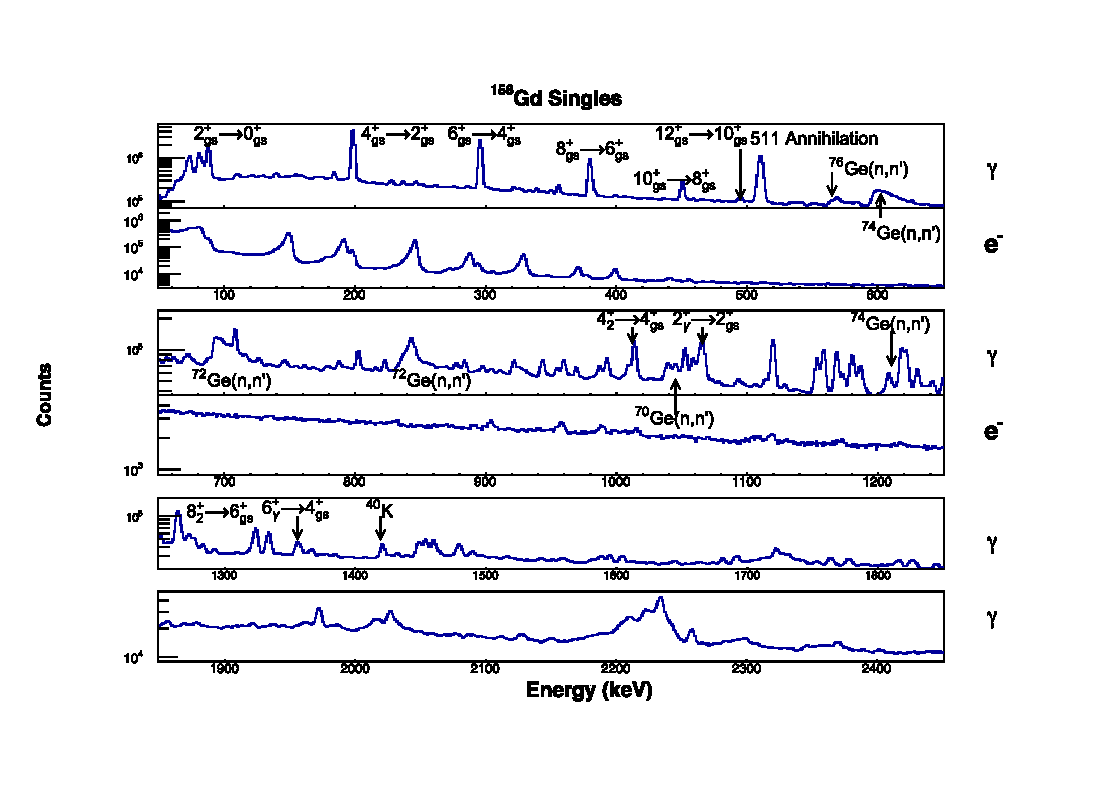
\includegraphics[scale=0.9]{156GdTablesAndFigs/156Gd_Singles_Label.eps}
    \caption{Singles spectra of $^{156}$Gd. Spectra are labeled with the particles being detected, the energies of the $\gamma$ and electron spectra aligned for identification. In the $\gamma$ spectrum, several lines of note are labeled. These are the ground-state band lines as well as other transitions of interest. Below 100 keV is a combination of x-rays and the 89 keV gamma from the ground state band. In the conversion electron spectrum, the large peaks up to approximately 350 keV are from the ground state band. These large peaks make the ground state band a good diagnostic, but also emphasize the need for coincidence gating, as the conversion electron spectrum is flooded by the ground state band electrons. The large peak at low energy is cut off due to the threshold. It is a combination of background and the 89L peak. Transitions in the higher energy regime of the $\gamma$ spectrum cannot be determined without gating, due to additional background from the experimental room.}
    \label{fig:156_Singles}
\end{figure}}

The transitions in the ground state band are used as a diagnostic of the data. The ground state band transitions should all be pure E2 multipole transitions and have been measured as such, making them aan excellent comparison and calibration with the theoretical coefficients from BrIcc\citep{kibedi08:_BRICC}. Singles data had to be corrected for angular distribution effects, discussed in section \ref{sec:angular}. The transitions from $2^+$ to $10^+$ are summarized and compared with theory in Table \ref{tab:156Gd_Single_ICC_GS}.

\afterpage{\begin{landscape}
\footnotesize
    \begin{longtable}{c|c|c|c|c|c|c|c|c|c}
    \caption{$^{156}$Gd Ground State Band Internal Conversion Coefficients from Singles}
        \label{tab:156Gd_Single_ICC_GS}\\
    \toprule
$E$ (keV)	&	$J^{\pi}	\rightarrow	J^{\pi}$	&	$E_i$ (keV)	&	$E_f$ (keV)	&	$T_{1/2}$ (fs)	&	Multipolarity	&	Shell & $\alpha$ (This Work)	&	$\alpha$  (Th)	&	$\alpha$ (Konijn)	\\
\hline		
\endfirsthead
    \caption[]{$^{156}$Gd Ground State Band Internal Conversion Coefficients from Singles}\\
    \toprule
$E$ (keV)	&	$J^{\pi}	\rightarrow	J^{\pi}$	&	$E_i$ (keV)	&	$E_f$ (keV)	&	$T_{1/2}$ (fs)	&	Multipolarity	&	Shell & $\alpha$ (This Work)	&	$\alpha$  (Th)	&	$\alpha$ (Konijn)	\\
\hline		
\endhead
\endfoot
\multicolumn{10}{p{1.4\textwidth}}{A list of the ground state conversion coefficients from $^{156}$Gd. Multipolarities and mixing ratios were taken from NNDC. Unless otherwise stated, the $\alpha$ values are $\alpha_K$. An angular distribution correction has been applied based on multipolarities for pure transitions, and those with known mixing ratios. The first error is statistical, the second is systematic. Numbers are compared with Konijn et al. \citep{konijn81:_156gd} Starred values in the Konijn data were used as calibration points.}
\endlastfoot
198.58	&	$4^+	\rightarrow	2^+$	&	288.187	&	88.97	&	111900	&	E2	& K &	0.1667 (4)$^{+46}_{-45}$	&	0.1565 (22)	&	0.199 (36)	\\
	&				&		&		&		&		& L &	0.0537 (1)$^{+16}_{-15}$	&	0.0531 (8)	&		\\
	&			&		&		&		&		& M &	0.0170 (1) (5)	&	0.0122 (2)	&		\\ \hline
296.04	&	$6^+	\rightarrow	4^+$	&	584.715	&	288.187	&	15800	&	E2 & K	&	0.0572 (1) (18)	&	0.0477 (7)	&	0.04683*	\\
	&				&		&		&		&	& L	&	0.0121 (1) (4)	&	0.0115 (2)	&		\\
	&				&		&		&		&	& M	&	0.0036 (1) (1) &	0.0026 (1)	&		\\ \hline
379.92	&	$8^+	\rightarrow	6^+$	&	965.134	&	584.715	&	4320	&	E2 & K	&		0.0274 (1) (9)	&	0.0235 (4)	&	0.038 (10)	\\
	&				&		&		&		&	& L	&	0.0050 (1) (2)	&	0.0048 (1)	&		\\
	&				&		&		&		&	& M	&	0.0013 (1) (1)	&	0.0011 (1)	&		\\ \hline
450.64	&	$10^+	\rightarrow	8^+$	&	1416.078	&	965.134	&	1900	&	E2	& K &	0.0152 (2) (5)	&	0.01483 (21)	& 0.0145*		\\
	&				&		&		&		&	& L	&	0.0028 (1) (1)	&	0.00279 (4)	&		\\
	&				&		&		&		&	& M	&	0.0010 (1) (1)	&	0.000621 (9)	&		\\ 
\bottomrule
    \end{longtable}
\end{landscape}}

There do not appear to be contaminants in these ground state lines, outside of the $2_{gs}^+\rightarrow0_{gs}^+$ transition, unlike the $^{154}$Gd data. The $2^+_{gs}\rightarrow 0^+_{gs}$ transition is considered unreliable, as the low energy of the $\gamma$-ray puts it in the energy region where the efficiency decreases due to the attenuation of the photon before it reaches the active region of the detector. The change in efficiency in the HPGe detectors is steep in this region, leading to large uncertainty.

\section{Gates on the Ground State Band}

The transitions of the ground state band are the most prominent peaks in the spectra (Figure \ref{fig:156_Singles}). The $\gamma$-rays of these transitions were gated onto confirm the levels populated in the reaction. Figures \ref{fig:156_2to0}, \ref{fig:156_4to2}, \ref{fig:156_6to4}, and \ref{fig:156_8to6} are the result of these gates. The $4_{gs}^+\rightarrow2_{gs}^+$ gate has the most statistics to work with, due to the challenges the attenuation of the $2^+_{gs}\rightarrow0_{gs}^+$ transition posed. 

\afterpage{\clearpage\begin{figure}[!]
    \centering
    \begin{subfigure}{\textwidth}
    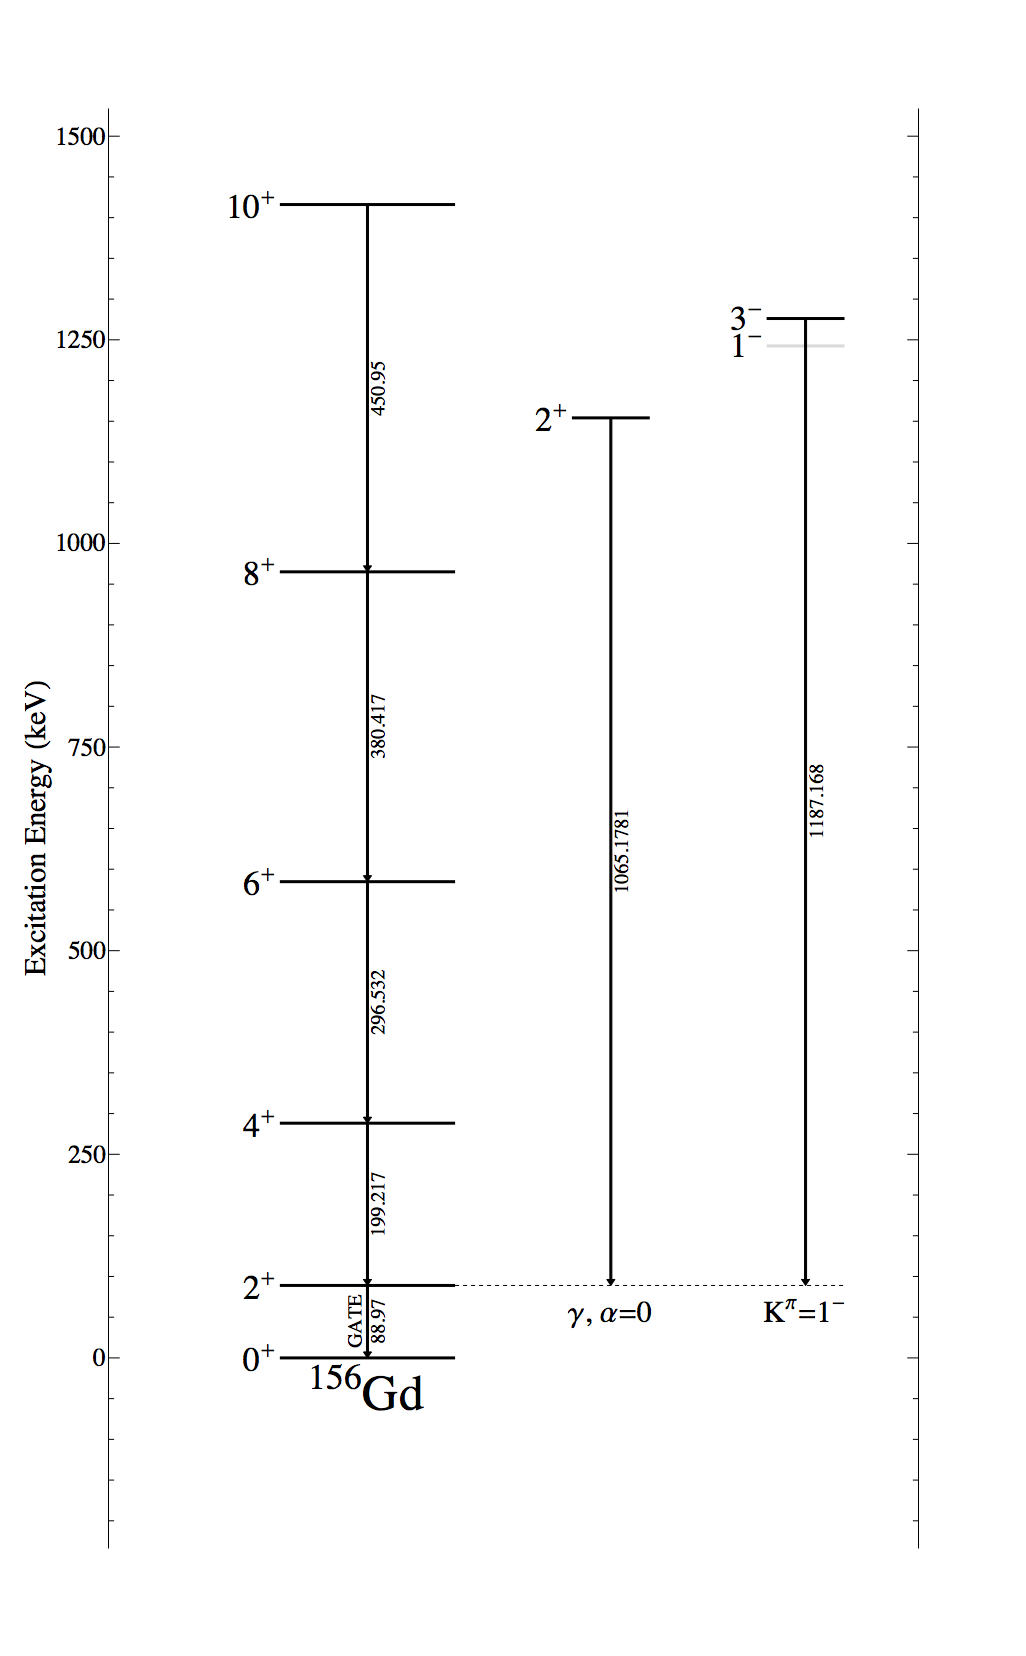
\includegraphics[scale=0.4]{156GdTablesAndFigs/156Gd_2to0.eps}
    \caption{\label{fig:156_2to0level}Level Scheme of $^{156}$Gd. The gamma ray of the $2^+$\rightarrow$0^+$ (89 keV) transition in the ground state was gated on. It was then compared with the gated spectrum from the gamma ray of the $4^+$\rightarrow$2^+$ (199 keV) transition in the ground state. Peaks only appearing in the first gate were assumed to go into the $2^+$ state, and assignments were made. Due to the low energy of the $2^+$\rightarrow$0^+$ transition, the efficiency was lower, and it is likely that transitions into the $2^+$ state were missed. The levels are organized by band. The lower levels of the band, unseen by gamma rays in this gate, are in gray.}
    \end{subfigure}
    \captionlistentry{Level scheme and spectrum of $^{156}$Gd based on the $2^+\rightarrow0^+$ transition.}
    \label{fig:156_2to0}
    \end{figure}
\begin{landscape}
    \begin{figure}
    \ContinuedFloat
    \begin{subfigure}{1.4\textwidth}
    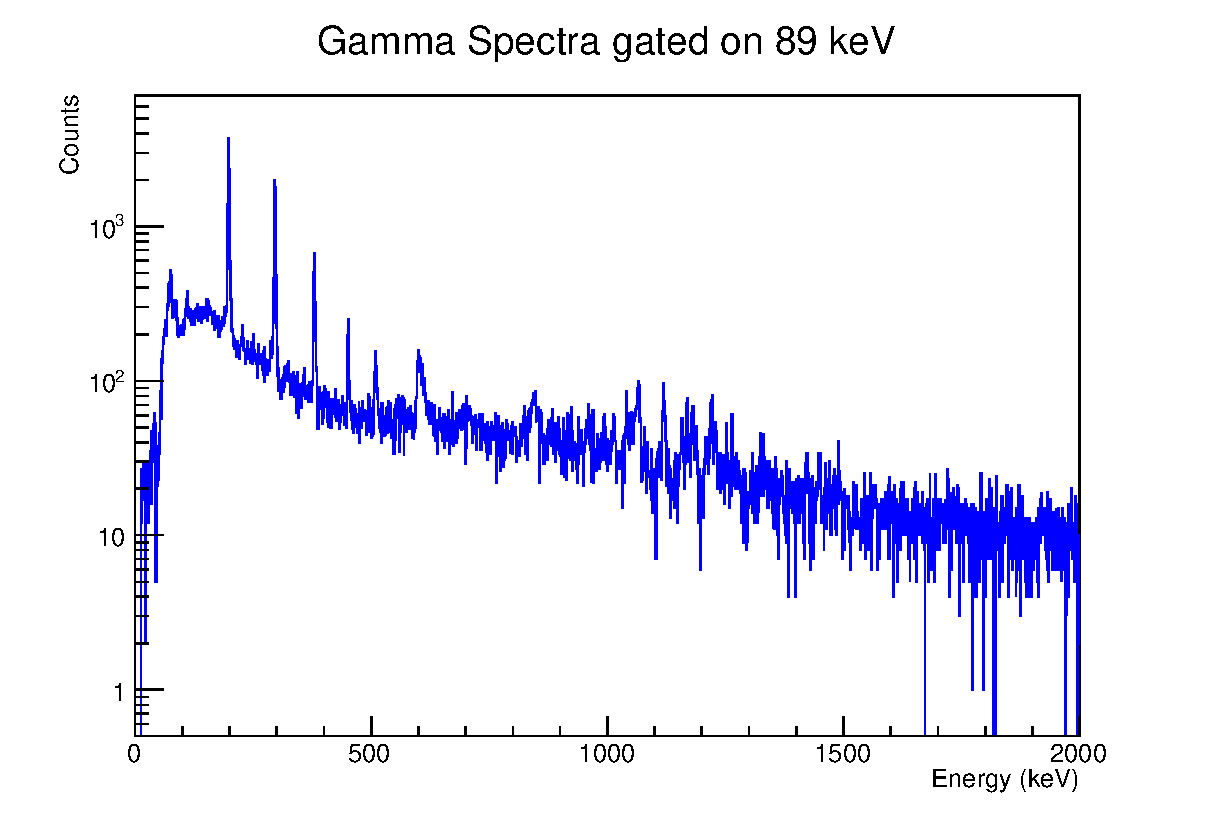
\includegraphics[]{156GdTablesAndFigs/89GateSpectrum.eps}
    \caption{Gamma spectrum gated on 89 keV, corresponding to the $2^+\rightarrow0^+$ transition.}
    \label{fig:156_2to0spec}
    \end{subfigure}
\end{figure}
\end{landscape}}

\afterpage{\clearpage\begin{landscape}
\begin{figure}
    \centering
    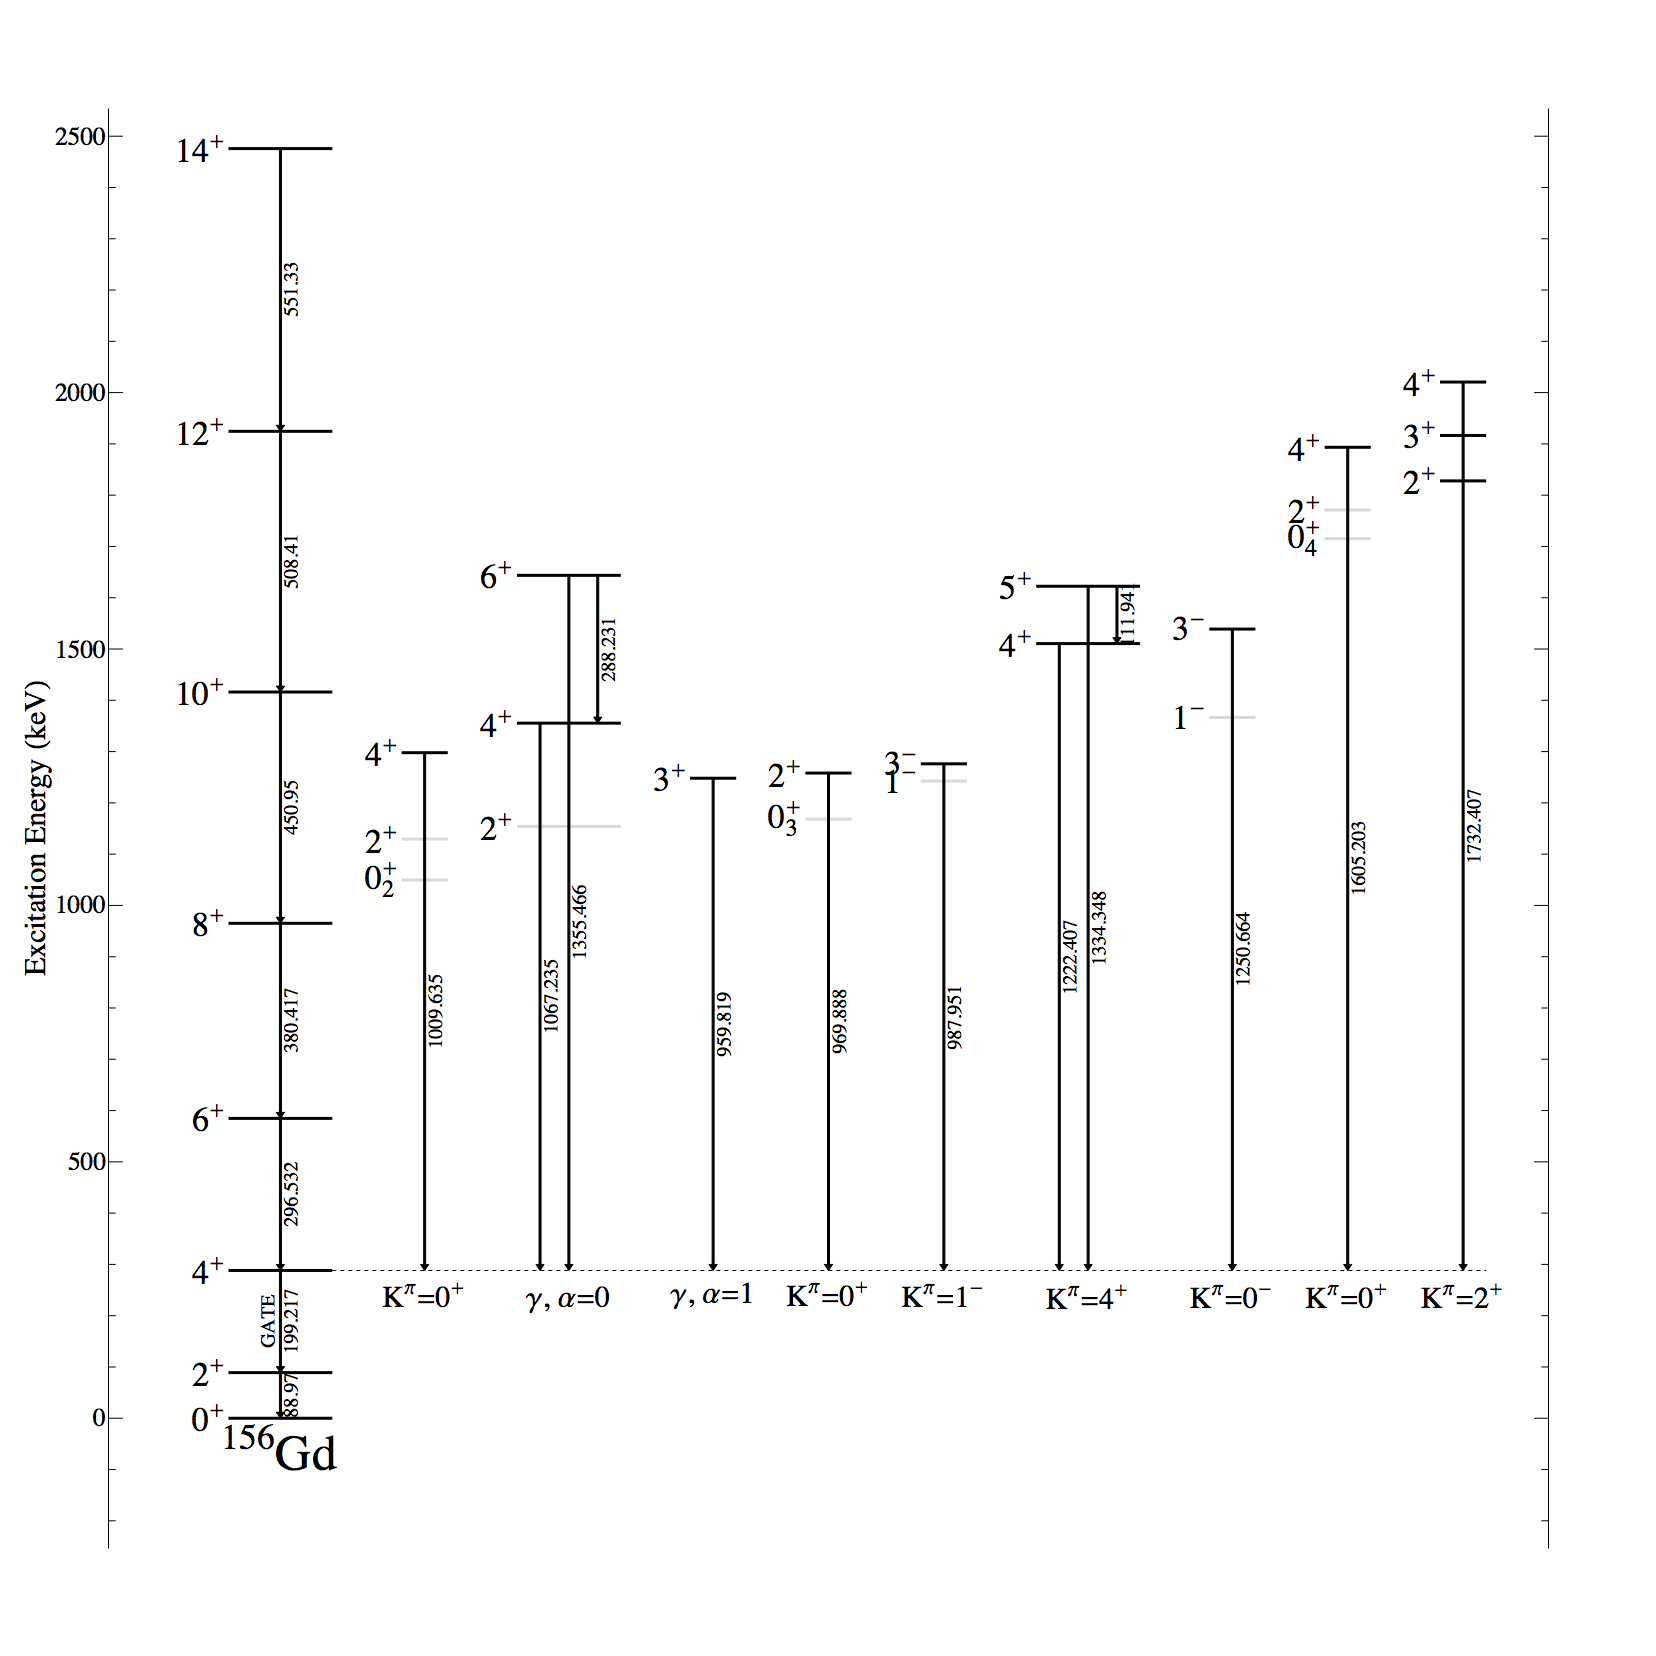
\includegraphics[scale=0.4]{156GdTablesAndFigs/156Gd_4to2.eps}
    \caption{Level Scheme of $^{156}$Gd. The gamma ray of the $4^+$\rightarrow$2^+$ (199 keV) transition in the ground state was gated on. It was then compared with the gated spectrum from the gamma ray of the $6^+$\rightarrow$4^+$ (296 keV) transition in the ground state. Peaks only appearing in the first gate were assumed to go into the $4^+$ state, and assignments were made. Additionally, these peaks were also gated on, to look for cascades leading into the $4^+$ state, which were found in several cases. The levels are organized by band. The lower levels of the band, unseen by gamma rays in this gate, are in gray.}
    \label{fig:156_4to2}
\end{figure}
\end{landscape}}

\afterpage{\clearpage\begin{figure}
    \centering
    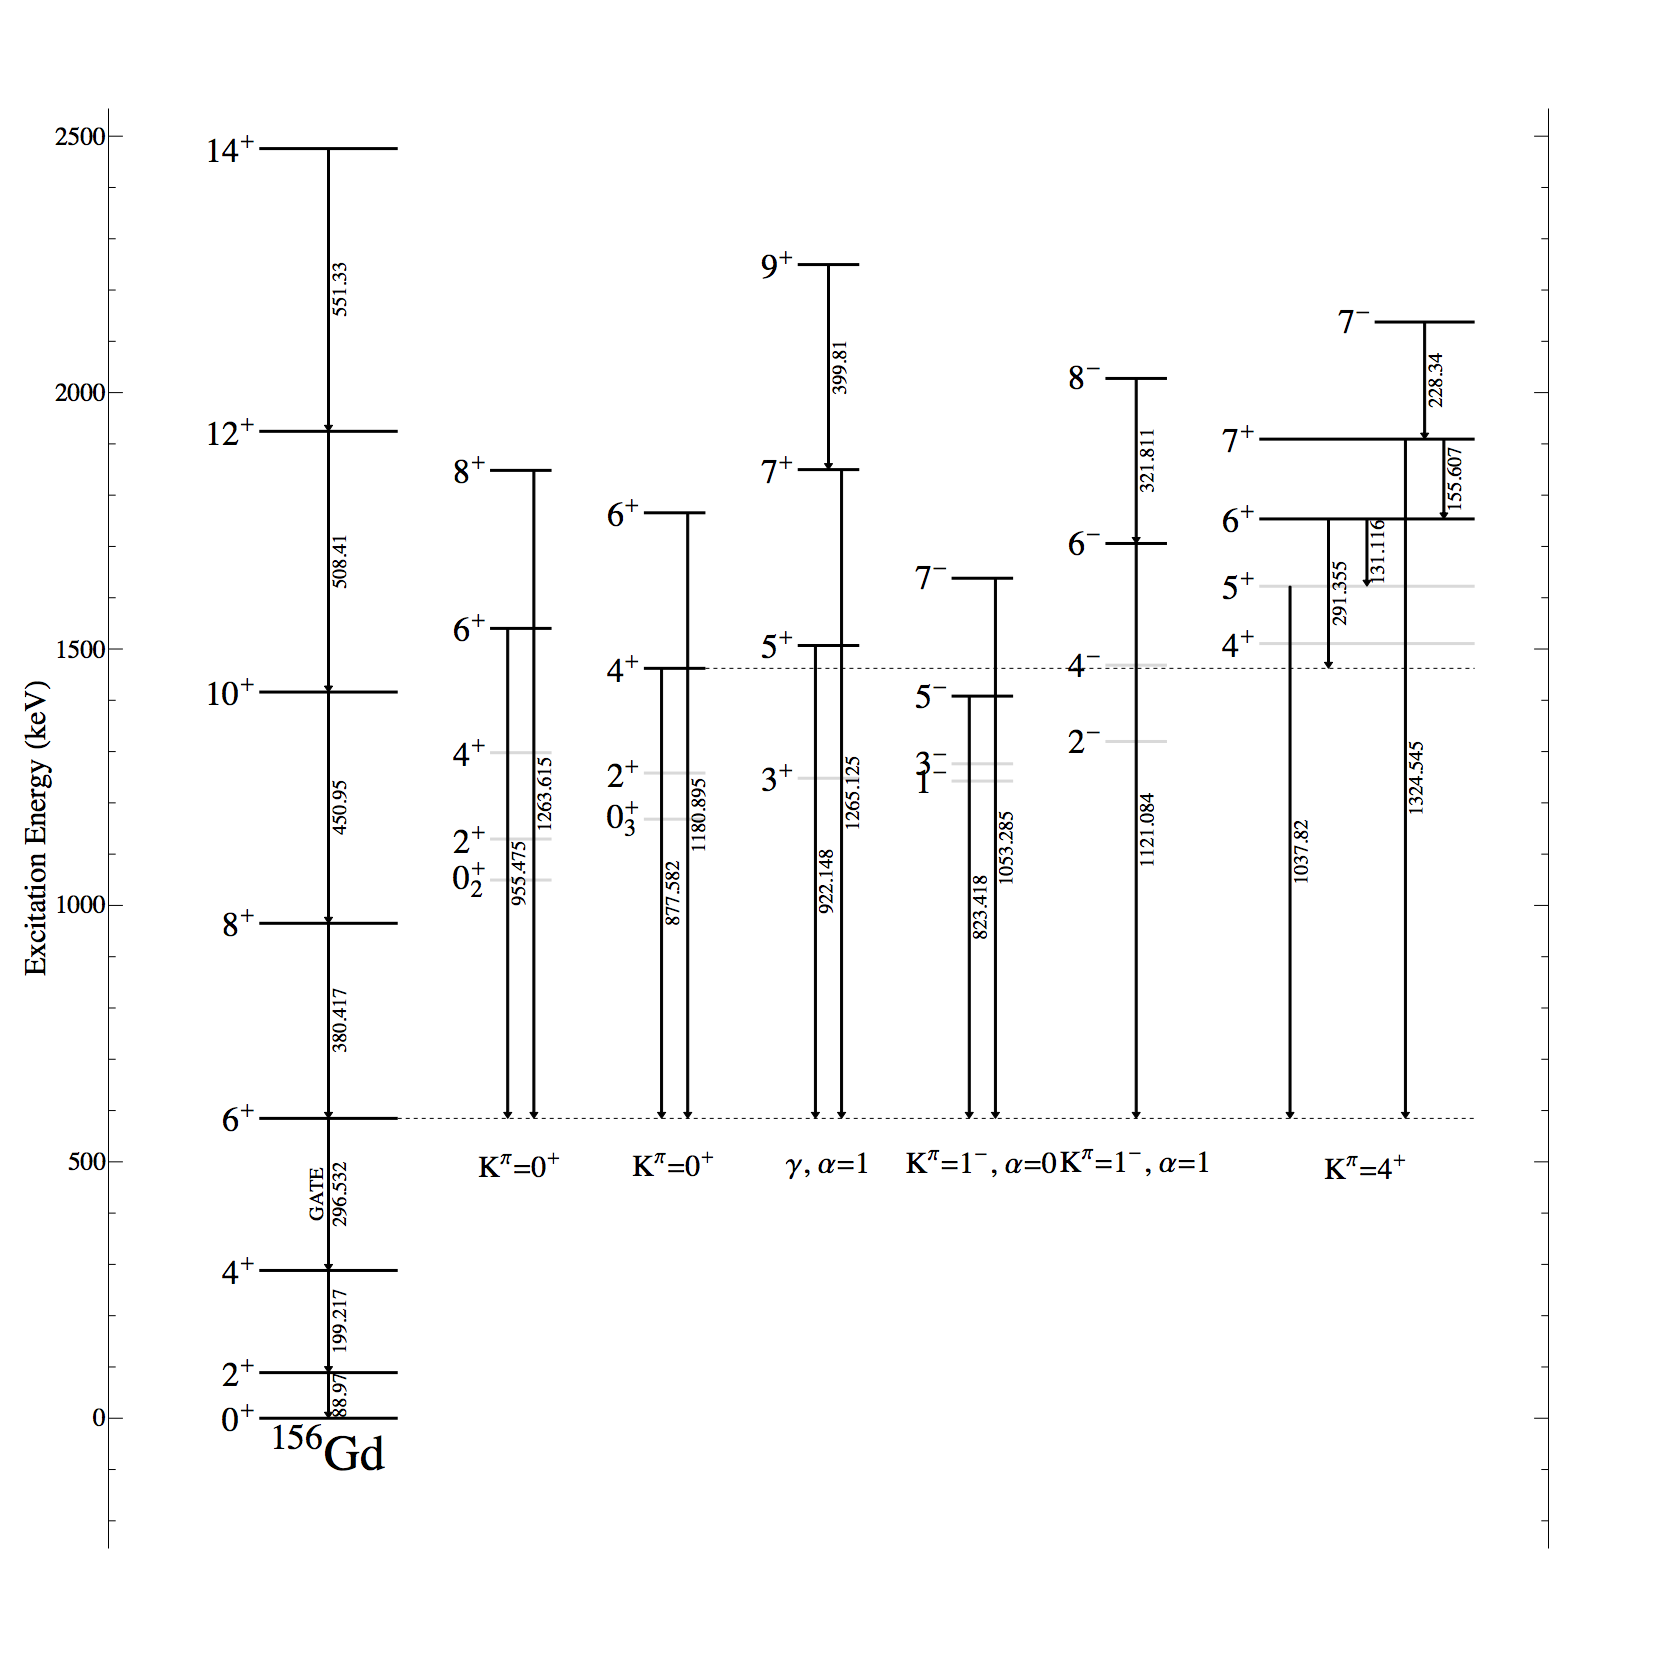
\includegraphics[scale=0.28]{156GdTablesAndFigs/156Gd_6to4.png}
    \caption{Level Scheme of $^{156}$Gd. The gamma ray of the $6^+$\rightarrow$4^+$ (296 keV) transition in the ground state was gated on. It was then compared with the gated spectrum from the gamma ray of the $8^+$\rightarrow$6^+$ (380 keV) transition in the ground state. Peaks only appearing in the first gate were assumed to go into the $6^+$ state, and assignments were made. Additionally, these peaks were also gated on, to look for cascades leading into the $6^+$ state, which were found in several cases. The levels are organized by band. The lower levels of the band, unseen by gamma rays in this gate, are in gray.}
    \label{fig:156_6to4}
\end{figure}}

\afterpage{\clearpage\begin{figure}
    \centering
    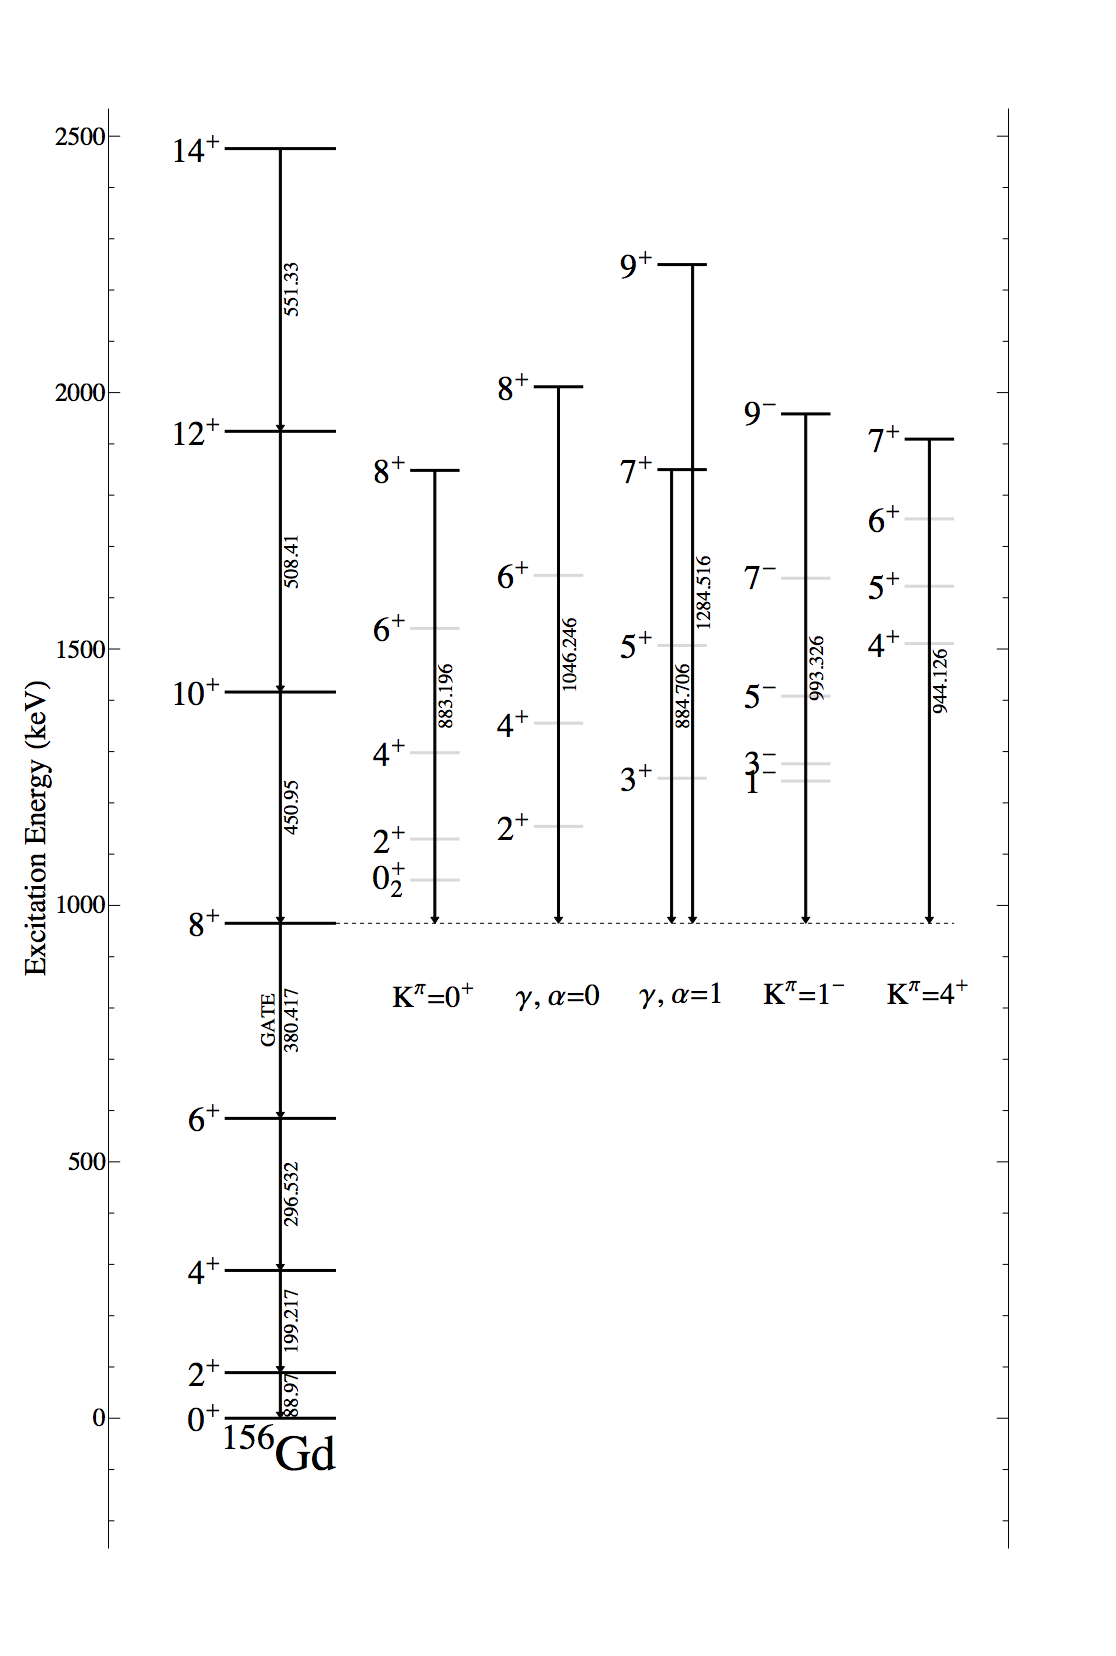
\includegraphics[scale=0.3]{156GdTablesAndFigs/156Gd_8to6.png}
    \caption{Level Scheme of $^{156}$Gd. The gamma ray of the $8^+$\rightarrow$6^+$ (380 keV) transition in the ground state was gated on. It was then compared with the gated spectrum from the gamma ray of the $10^+$\rightarrow$8^+$ (451 keV) transition in the ground state. Peaks only appearing in the first gate were assumed to go into the $8^+$ state, and assignments were made. Additionally, these peaks were also gated on, to look for cascades leading into the $8^+$ state, which were found in several cases. The levels are organized by band. The lower levels of the band, unseen by gamma rays in this gate, are in gray.}
    \label{fig:156_8to6}
\end{figure}}

Determining which transitions went uniquely into a given ground state level was done by comparing the outgoing ground state transition for that level with the incoming transitions, i.e. the $4_{gs}^+\rightarrow2_{gs}^+$ (199 keV) gate was compared directions with the $6_{gs}^+\rightarrow4_{gs}^+$ (296 keV) gate. The $\gamma$-spectra corresponding to gates of two of these lines can be seen in Figure \ref{fig:156_GS_Gate}. Lines in the gamma spectrum that were present only in the outgoing spectrum, but not the incoming spectrum, are going into that level (the $4_{gs}^+$ in the example above). Several areas have been circled to demonstrate this effect. Identified transitions were then gated on to confirm assignments and search for cascades from higher energy states.

\begin{figure}[!]
    \centering
    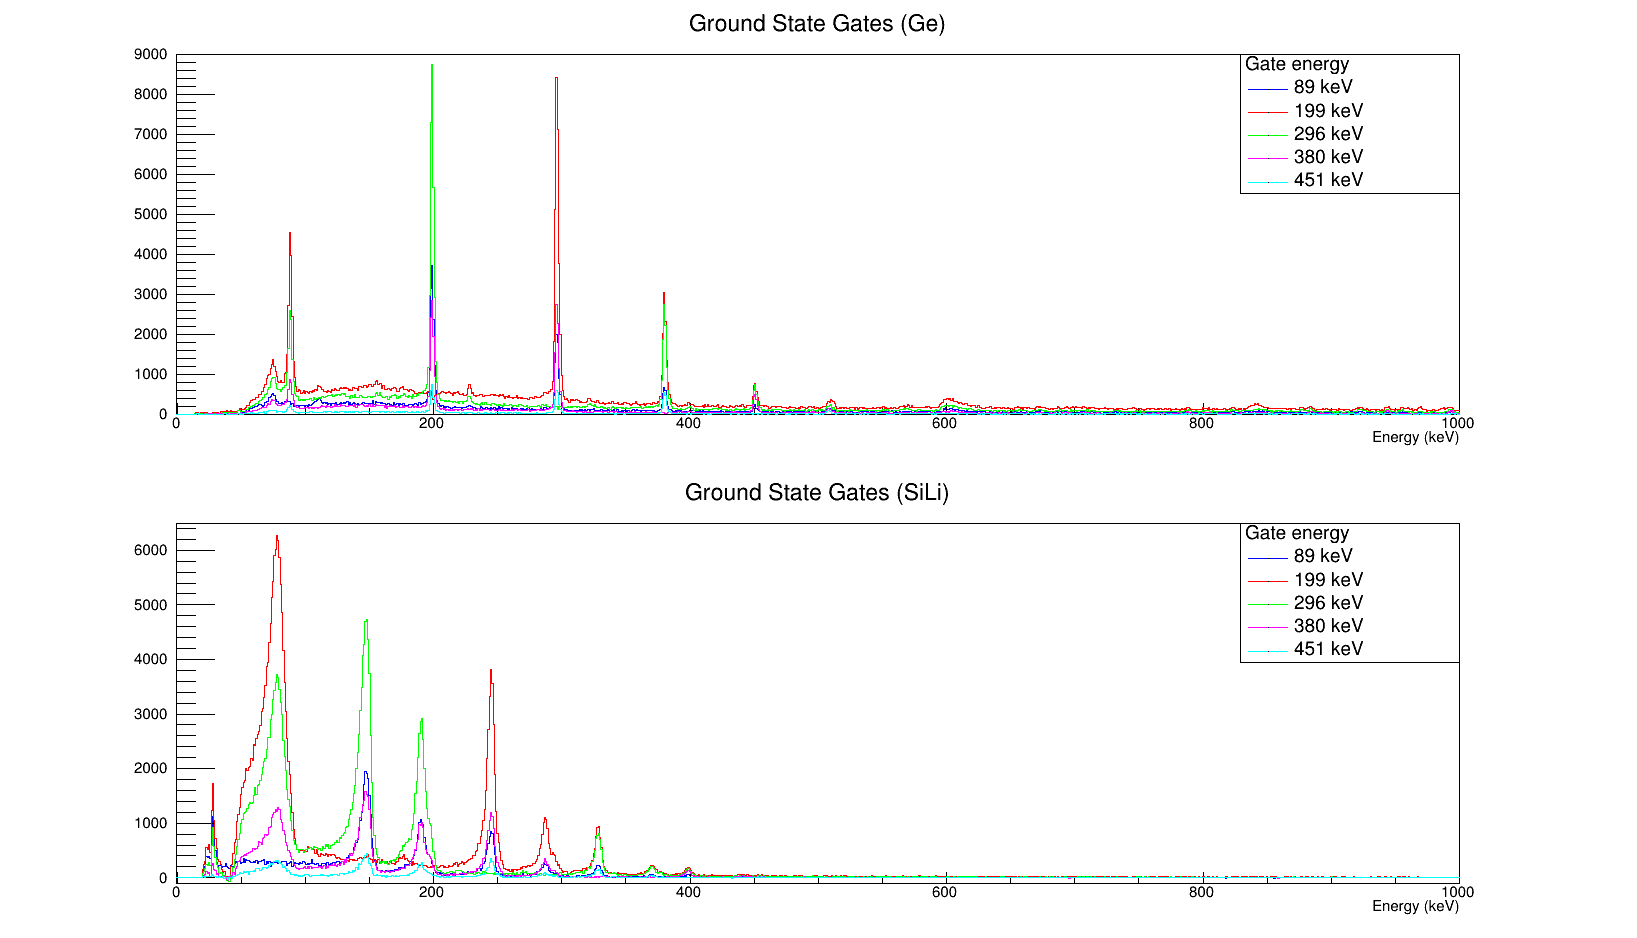
\includegraphics[scale=0.27]{156GdTablesAndFigs/156GS_stack.png}
    \caption{Spectra gated on the ground state band lines of $^{156}$Gd. As can be seen, some lines do not appear in different gates. Comparison of these gates, for instance 199 keV ($4^+\rightarrow2^+$) and 296 keV ($6^+\rightarrow4^+$), yields a list of transitions that directly populate the interim level (in the example, the $4^+$ state). The 89 keV line, although the lowest transition in the ground state band, has a low yield due to efficiency, and is reflected in the relative size of the peaks. The 199 keV peak in the gamma spectrum is much larger from the 296 keV transition than the 89 keV transition.}
    \label{fig:156_GS_Gate}
\end{figure}

The secondary gate check is important, as the attenuation of the $2_{gs}^+\rightarrow0_{gs}^+$ transition meant weaker lines going into the $2_{gs}^+$ state could be falsely assigned going into the $4_{gs}^+$ state. As the ground state band transitions are so intense, the transitions showed up when gating on weaker peaks in the spectra, while the inverse was not always true. The spectra from these gates are available in Appendix \ref{chap:156_spectra}.

Few transitions could be seen in the $2_{gs}^+\rightarrow0_{gs}^+$ (89 keV) gate, as is reflected in Figure \ref{fig:156_2to0}. The $4_{gs}^+\rightarrow2_{gs}^+$ (199 keV) gate shows a larger number of $\gamma$-rays, seen in Figure \ref{fig:156_4to2}, including evidence of populating 3 excited $0^+$ bands. In total, nine bands were seen in the gating. The number of bands seen populated drops off with higher gates, both due to the drop off in populating higher energy states and the drop off in populating higher $J$ states. Studies have shown the $(\alpha,2n)$ reaction to stop populating spin states with a significant cross section beyond about $J^{\pi}=12^+$ \citep{wu93:_a2n}. In the ground state band of $^{156}$Gd, the $12^+_{gs}$ state sits at 1924.49 keV, giving an approximate cut off for populating higher energy states in the nucleus. Additionally, due to the lack of known higher spin states in the higher energy $0^+$ bands, identification of populating the bands in the higher gates becomes difficult.

\section{Conversion Coefficients from Singles}

With the gamma-rays now identified through gates, conversion coefficients could be calculated from singles spectra. Tables \ref{tab:156Gd_Single_ICC_Corr}, \ref{tab:156Gd_Single_ICC_Uncorr}, and \ref{tab:156Gd_No_Mult_ICC} are these results. Where available, results are compared with Konijn et al\citep{konijn81:_156gd}, which also examined the nucleus via an $(\alpha,2n)$ reaction.

Transitions that could be clearly identified and distinguished are found in Table \ref{tab:156Gd_Single_ICC_Corr}. These transitions all have known multipole assignments and mixing ratios as needed, allowing for angular corrections. Two transitions with possible E0 components are seen in this table. One, the $2^+_{0^+_{2}}\rightarrow 2^+_{gs}$ transition, appears to have a clear E0 component. Although this transition was not seen in Figure \ref{fig:156_2to0}, the band the state exists in is populated, as seen in Figures \ref{fig:156_4to2}, \ref{fig:156_6to4}, and \ref{fig:156_8to6}. The $6^+_{\gamma}\rightarrow 6^+_{gs}$ transition does not appear to have an E0 component. While the value agrees with Konijn\citep{konijn81:_156gd}, it does not agree with the theoretical value for an E2, the multipole the transition has been assigned.

\afterpage{\clearpage\begin{landscape}
    \begin{longtable}{>{\footnotesize}c|>{\footnotesize}c|>{\footnotesize}c|>{\footnotesize}c|>{\footnotesize}c|>{\footnotesize}c|>{\footnotesize}c|>{\footnotesize}c|>{\footnotesize}c|>{\footnotesize}c|>{\footnotesize}c}
    \caption{$^{156}$Gd Internal Conversion Coefficients from Singles}
        \label{tab:156Gd_Single_ICC_Corr}\\
    \toprule
$E$ (keV)	&	$J^{\pi}	\rightarrow	J^{\pi}$	&	$E_i$ (keV)	&	$E_f$ (keV)	&	$T_{1/2}$ (fs)	&	Multipolarity	&	$\delta$	& Shell &	$\alpha$ (This Work)	&	$\alpha$  (Theory)\citep{kibedi08:_BRICC}	&	$\alpha$ (Konijn)\citep{konijn81:_156gd}	\\
\hline		
\endfirsthead
    \caption[]{$^{156}$Gd Internal Conversion Coefficients from Singles}\\
    \toprule
$E$ (keV)	&	$J^{\pi}	\rightarrow	J^{\pi}$	&	$E_i$ (keV)	&	$E_f$ (keV)	&	$T_{1/2}$ (fs)	&	Multipolarity	&	$\delta$ & Shell &	$\alpha$ (This Work)	&	$\alpha$  (Theory)\citep{kibedi08:_BRICC}	&	$\alpha$ (Konijn)\citep{konijn81:_156gd}	\\
\hline		
\endhead
\endfoot
\multicolumn{11}{p{1.4\textwidth}}{A list of conversion coefficients from $^{156}$Gd. Multipolarities and mixing ratios were taken from the nuclear date sheets\citep{reich12:_nds_156}. Unless otherwise stated, the $\alpha$ values are $\alpha_K$. An angular distribution correction has been applied based on multipolarities for pure transitions, and those with known mixing ratios. The first error is statistical, the second is systematic. Numbers are compared with Konijn et al\citep{konijn81:_156gd}.}
\endlastfoot
227.90	&	$7^-_{7^-}	\rightarrow 7^+_{4^+}$	&	2137.6	&	1909.26	&	1300000000	&	E1	&	& K	&	0.4687 (50)$^{+85}_{-84}$	&	0.0272 (4)	&	0.063 (13)	\\
	&			&		&		&		&		&	& LM	&	0.1073 (20) (20)	&	0.0049 (6)	&		\\ \hline
321.92	&	$8^-_{1^-}	\rightarrow	6^-_{1^-}$	&	2027.1	&	1705.799	&		&	E2	&		& K &	0.0290 (13) (9)	&	0.0378 (6)	&	0.025 (7)	\\ \hline
355.87	&	$4^+_{4^+}	\rightarrow	2^+_{\gamma}$	&	1510.594	&	1154.152	&	189000	&	E2	&		& K &	0.0158 (6) (5)	&	0.0281 (4)	&	\\ \hline
399.56	&	$9^+_{\gamma}	\rightarrow	7^+_{\gamma}$	&	2249.65	&	1849.84	&		&	E2	&		& K &	0.0077 (8) (3)	&	0.0205 (3)	&	0.026 (5)	\\ \hline
921.83	&	$5^+_{\gamma}	\rightarrow	6^+_{gs}$	&	1506.863	&	584.715	&	400	&	E2	&		& K &	0.0041 (9) (5) &	0.0028 (1)	&	0.0030 (7)	\\ \hline
1040.470	&	$2^+_{0^+_{2}}	\rightarrow	2^+_{gs}$	&	1129.437	&	88.970	&		&	E2+E0+M1	&	$-5.9^{+14}_{-28}$	& K &	0.0152 (10) (2)	&	0.0022 (1)	&	0.014 (3)	\\ \hline
1059.31	&	$6^+_{\gamma}	\rightarrow	6^+_{gs}$	&	1643.653	&	584.715	&		&	E2	&		& K &	0.0013 (5) (1)	&	0.0021 (1)	&	0.0013 (8)	\\ \bottomrule
    \end{longtable}
\end{landscape}}

Table \ref{tab:156Gd_Single_ICC_Uncorr} holds conversion coefficients that have been left uncorrected for angular distribution in the singles for one of two reasons: either there were multiple known assignments to the gamma-ray energy, or the exact multipole mixing-ratio $\delta$ was unknown. Several of these transitions are high energy $J^\pi\rightarrow J^\pi$ transitions, including a $0^+\rightarrow0^+$ transition. The Si(Li) efficiency at these energies was too low to see the conversion electrons in gated spectra.

\afterpage{\clearpage	\begin{ThreePartTable}
		\begin{longtable}{>{\footnotesize}c|>{\footnotesize}c|>{\footnotesize}c|>{\footnotesize}c|>{\footnotesize}c|>{\footnotesize}c|>{\footnotesize}c}
			\caption{Uncorrected $^{156}$Gd Internal Conversion Coefficients from Singles\label{tab:156Gd_Single_ICC_Uncorr} }\\
			\multicolumn{6}{c}{(a)} \\
			\toprule
	& & & & & \\
	$E$ (keV)	&	$J^{\pi}	\rightarrow	J^{\pi}$	&	$E_i$ (keV)	&	$E_f$ (keV)	& $T_{1/2}$ (fs) &	Multipolarity	&	$\delta$ \\
	\hline
	\endfirsthead
	\caption[]{Uncorrected $^{156}$Gd Internal Conversion Coefficients from Singles} \\
	\multicolumn{6}{c}{(a)} \\
	\toprule
	$E$ (keV)	&	$J^{\pi}	\rightarrow	J^{\pi}$	&	$E_i$ (keV)	&	$E_f$ (keV)	& $T_{1/2}$ (fs) &	Multipolarity	&	$\delta$ \\
	\hline
	\endhead
154.94	&	$4^+_{4^+}	\rightarrow	4^+_{\gamma}$	&	1510.594	&	1355.422	&	189000	&	M1+E2	&	0.48	\\
	&	$7^+_{4^+}	\rightarrow	6^+_{4^+}$	&	1909.26	&	1753.653	&		&	(M1+E2)	&	0.29	\\ \hline
883.86	&	$8^+_{0^+_{2}}	\rightarrow	8^+_{gs}$	&	1848.33	&	965.134	&		&	E0+E2	&		\\
	&	$7^+_{\gamma}	\rightarrow	8^+_{gs}$	&	1849.84	&	965.134	&		&	E2(+M1)	&		\\ 
	&		&		&	&		&	\\ \hline
955	&	$6^+_{0^+_{2}}	\rightarrow	6^+_{gs}$	&	1540.19	&	584.715	&		&	E0+E2	&		\\ 
959.88	&	$0^+_{0^+_{2}}	\rightarrow	2^+_{gs}$	&	1049.487	&	88.97	&	1800	&	E2	&			\\
	&	$3^+_{\gamma}	\rightarrow	4^+_{gs}$	&	1248.006	&	288.197	&	580	&	E2+M1	&	-12	\\ \hline
1009.33	&	$4^+_{0^+_{2}}	\rightarrow	4^+_{gs}$	&	1297.822	&	288.197	&	1600	&	E0+E2,M1	&		\\ 
&		&		&	&		&	\\ \hline
1045.48	&	$8^+_{\gamma}	\rightarrow	8^+_{gs}$	&	2011.38	&	965.134	&		&	E2(+M1)	&		\\ 
&		&		&	&		&	\\ 
1052.61	&	$7^-_{1^-}	\rightarrow	6^+_{gs}$	&	1638	&	584.715	&		&	E1	&		\\ \hline
1065.74	&	$2^+_{\gamma}	\rightarrow	2^+_{gs}$	&	1154.152	&	88.97	&	568	&	E2+M1	&	-16	\\
	&	$4^+_{\gamma}	\rightarrow	4^+_{gs}$	&	1355.422	&	288.187	&	540	&	E2+M1	&	-4	\\ \hline
1158.65	&	$2^+_{\gamma}	\rightarrow	0^+_{gs}$	&	1154.152	&	0	&	568	&	E2	&		\\
	&	$3^+_{\gamma}	\rightarrow	2^+_{gs}$	&	1248.006	&	88.97	&	580	&	E2+M1	&	-11.8	\\ \hline
1168.69	&	$0^+_{0^+_{3}}	\rightarrow	0^+_{gs}$	&	1168.186	&	0	&	5000	&	E0	&		\\
	&	$2^+_{0^+_{3}}	\rightarrow	2^+_{gs}$	&	1258.075	&	88.97	&	1540	&	E2+M1+E0	&	0.38	\\ \hline
1222.22	&	$4^+_{4^+}	\rightarrow	4^+_{gs}$	&	1510.594	&	288.197	&	189000	&	M1+E2	&	-1.7	\\
	&	$5^+_{\gamma}	\rightarrow	4^+_{gs}$	&	1506.863	&	288.197	&	400	&	E2	&		\\ \hline
1264.85	&	$4^+_{\gamma}	\rightarrow	2^+_{gs}$	&	1355.422	&	88.97	&	540	&	E2	&		\\
	&	$8^+_2	\rightarrow	6^+_{gs}$	&	1848.33	&	584.715	&		&		\\
	&	$7^+_{\gamma}	\rightarrow	6^+_{gs}$	&	1849.84	&	584.715	&		&		\\ 
	&		&		&	&		&	\\ 
	\bottomrule
\end{longtable}
\end{ThreePartTable}
\pagebreak
\begin{ThreePartTable}
	\begin{TableNotes}[para]
		Table \ref{tab:156Gd_Single_ICC_Uncorr}: A list of conversion coefficients from $^{156}$Gd. Multipolarities and mixing ratios were taken from the nuclear data sheets\citep{reich12:_nds_156}. Unless otherwise stated, the $\alpha$ values are $\alpha_K$. No angular distribution correction has been applied, either due to unknown mixing ratios, or multiple assignments of the gamma-ray. The first error is statistical, the second is systematic. Numbers are compared with Konijn et al. \citep{konijn81:_156gd} Starred values were used as calibration points in the Konijn paper. All coefficients are K-shell electrons.
	 \end{TableNotes}
\begin{longtable*}{>{\footnotesize}c|>{\footnotesize}c|>{\footnotesize}c|>{\footnotesize}c|>{\footnotesize}c|>{\footnotesize}c}
	%\multicolumn{6}{c}{\MakeUppercase{Table \ref{tab:156Gd_Single_ICC_Uncorr} (Continued)}} \\
	\multicolumn{6}{c}{\MakeUppercase{Table 5.4 (Continued)}} \\
	\multicolumn{6}{c}{(b)} \\
	\toprule
	&  & \multicolumn{2}{>{\footnotesize}c|}{$\alpha$ (This Work)} & & \\
	$E$ (keV)	& Shell	&	Uncorrected & Corrected &	$\alpha$  (Th)\citep{kibedi08:_BRICC}	&	$\alpha$ (Konijn)\citep{konijn81:_156gd} \\
	\hline
	\endfirsthead
	%\multicolumn{6}{c}{\MakeUppercase{Table \ref{tab:156Gd_Single_ICC_Uncorr} (Continued)}} \\
	\multicolumn{6}{c}{\MakeUppercase{Table 5.4 (Continued)}} \\
	\multicolumn{6}{c}{(b)} \\
	\toprule
	&  & \multicolumn{2}{>{\footnotesize}c|}{$\alpha$ (This Work)} & & \\
	$E$ (keV)	& Shell	&	Uncorrected & Corrected &	$\alpha$  (Th)\citep{kibedi08:_BRICC}	&	$\alpha$ (Konijn)\citep{konijn81:_156gd} \\
	\hline
	\endhead
	154.94	& K & 	0.4635 (183)$^{+98}_{-97}$	& 0.3462 (137)$^{+73}_{-72}$ &	0.460 (7)	& \\
	&		 K &	0.4879 (193)$^{+103}_{-102}$ &	0.474 (7)	&		\\ \hline
883.86	& K &	0.0057 (7) (1)	& 0.0034 (4) (1) &	0.0030 (1)	& $>0.0092$		\\
& K &		&	[M1] 0.0102 (13) (2) & [M1] 0.0052 (1)	&	$<0.0052$	\\ 
&  &		&	[E2] 0.0073 (9) (1) & [E2] 0.0030 (1)	&		\\ \hline
955	& K &	0.0065 (4) (5)	& 0.0039 (2) (3) &	0.0026 (1)	&	0.020 (8)	\\ 
959.88	& K & &	0.0136 (8) (10) &  0.0025 (1)	&	0.0045 (24)	\\
& K &		&	0.0120 (7) (9) & 0.0025 (1)	&		\\ \hline
1009.33	& K &	0.0173 (9) (4)	& [M1] 0.0234 (12) (5) &	[M1] 0.0038 (1)	&	0.0164 (29)	\\ 
&  &		&	[E2] 0.0107 (6) (2) & [E2] 0.0023 (1)	&		\\ \hline
1045.48	& K &	0.0012 (2) (2)	& [M1] 0.0015 (3) (3)	 & [M1] 0.0035 (1)	&	0.0025 (6)	\\ 
&  &		&	[E2] 0.0007 (1) (1) & [E2] 0.0021 (1)	&		\\ 
1052.61	& K & &  0.0008 (1) (1)	&	0.0009 (1)	&		\\ \hline
1065.74	& K &	0.0023 (2) (1)	& 0.0034 (3) (1) &	0.0021 (1)	&	0.0025 (9)	\\
& K &		&	0.0029 (3) (1) & 0.0021 (3)	&	0.0021 (1)	\\ \hline
1158.65	& K &	0.0020 (3) (1)	& 0.0020 (3) (1) &	0.0017 (1)	&	0.0023 (3)	\\
& K & & 0.0014 (2) (1)		&	0.0017 (1)	&		\\ \hline
1168.69	& K &	0.0045 (3) (1)	& 0.0045 (3) (1) & 		&	$>0.0035$	\\
& K &	& 0.0038 (3) (1)	&	0.0026 (1)	&		\\ \hline
1222.22	& K &	0.0028 (4) (1)	 & 0.0031 (4) (1) &	0.0018 (1)	&	0.00174*	\\
& K &		& 0.0031 (4) (1)	& 0.001560 (22)	&	\\ \hline
1264.85	& K &	0.0017 (3) (1) & 0.0014 (2) (1)	&	0.0014 (1)	&	\\
& K &		& [E2] 0.0014 (2) (1)	&	[E2] 0.0014 (1) &		\\
& K &		& [M1] 0.0011 (2) (1)	& [M1] 0.0022 (1)	&		\\ 
&		&		&	[E2] 0.020 (3) (1) & [E2] 0.0014 (1)	&		\\
	\bottomrule
	\insertTableNotes
\end{longtable*}

\end{ThreePartTable}}

Table \ref{tab:156Gd_No_Mult_ICC} has conversion coefficients that could not be corrected for angular distribution due to the transitions having unknown multipole assignments. Allowable and reasonable theoretical conversion coefficients from BrIcc\citep{kibedi08:_BRICC} are listed in the table. Assuming pure multipole assignments, corrected coefficients have also been listed for comparison. The $7^+_{4^+}\rightarrow 8^+_{gs}$ transition sits within the theoretical bounds of the conversion coefficients when corrected. Using equation \ref{eq:ICC_Subtract}, the E2+M1 mixing ratio delta comes out to be $<0.61$ or $-0.55^{+51}_{-8}$. This value is small enough to indicate this transition may be a pure E2 transition. 

\afterpage{\clearpage\begin{landscape}
    \begin{longtable}{c|c|c|c|c|c|c|c|c}
        \caption{$^{156}$Gd Internal Conversion Electrons without known Multipolarities}
        \label{tab:156Gd_No_Mult_ICC}\\
        \toprule
        &	& 	&  &	& \multicolumn{2}{c}{Theory}	& 	\\
        $E_i$ (keV)	&	$E_f$ (keV)	& $E$ (keV)	&	Gate &		$\alpha$ (This Work)	& $\alpha$(M1) & $\alpha$(E2) & $\alpha$(E1) &	$\alpha$ (Konijn)	\\
        \hline		
        \endfirsthead
        \caption[]{$^{156}$Gd Internal Conversion Electrons without known Multipolarities}\\
        \toprule
        &	& 	&  &	& \multicolumn{2}{c}{Theory}	& 	\\
        $E_i$ (keV)	&	$E_f$ (keV)	& $E$ (keV)	&	Gate &		$\alpha$ (This Work)	& $\alpha$(M1) & $\alpha$(E2) & $\alpha$(E1) &	$\alpha$ (Konijn)	\\
        \hline		
        \endhead
        671.41	&	$7^-	\rightarrow	8^+$	&	1638	&	965.134	&		0.0064 (6) (2)	& & & 0.00213 (3) &	\\ \hline
        838.83	&	$9^+	\rightarrow	10^+$	&	2249.65	&	1416.078	&	0.0009 (3) (1)	& 0.00595 (9) & 0.00337 (5) & & 	\\ \hline
        943.732	&	$7^+	\rightarrow	8^+$	&	1909.26	&	965.134		&	0.0022 (6) (1) & 0.00448 (7) & 0.00262 (4) & &	0.0025 (3)	\\ 
        \bottomrule
    \end{longtable}
    \caption{A list of conversion coefficients from $^{156}$Gd without known multipolarities. As a result, an angular distribution correction term has not been applied. None of the states have known half lives. The first error is statistical, the second is systematic. Numbers are compared with theoretical values for allowed multipolarities and results from Konijn et al. \citep{konjin81:_156gd}. All coefficients are K-shell electrons.}
\end{landscape}}

\section{$J^{\pi}\rightarrow J^{\pi}$ Transitions}

\subsection{$0^{+}\rightarrow 0^{+}$ Identification and Population}

With the large number of $0^+$ states in $^{156}$Gd, our first priority was to identify which bands were populated. Table \ref{tab:0plus_156} contains a list of $0^+$ states from the nuclear data sheets \citep{reich12:_nds_156}, with notes as to which $0^+$ states have been previously observed in the reaction used in this work.

\begin{table}[]
    \centering
    \caption{$0^+$ States in $^{156}$Gd}
    \label{tab:0plus_156}
    \begin{tabular}{c|c|c}
        Energy (keV) &  Seen in $(\alpha,2n)$ & Seen in This Work  \\
        \toprule
        0 & $\times$ & $\times$\\
        1049.487(2) & $\times$ & $\times$\\
        1168.186(7) & $\times$ & $\times$\\
        1715.211(4) & & $\times$\\
        1851.278(7) & & $\times$\\
        1988.5(2) & & \\
        2082.0 & & \\
        \bottomrule
    \end{tabular}
\end{table}

We have seen all $0^+$ states observed previous in $(\alpha,2n)$ experiments in addition to two more of higher energy. The energies of the possible $0^+\rightarrow 0^+$ transitions from these states are marked in the electron singles in Figure \ref{fig:156_e_singles}. In this spectrum, the $0^+_{3}\rightarrow 0^+_{gs}$ transition is the most prominent. The $0^+_{2}\rightarrow 0^+_{gs}$ and $0^+_{4}\rightarrow 0^+_{3}$ transitions appears to have some strength, but are obscured by other conversion electrons in the data. The $0^+_{3}\rightarrow 0^+_{2}$ transition is at too low an energy to distinguish from the high background at low energies.

\begin{figure}
    \centering
    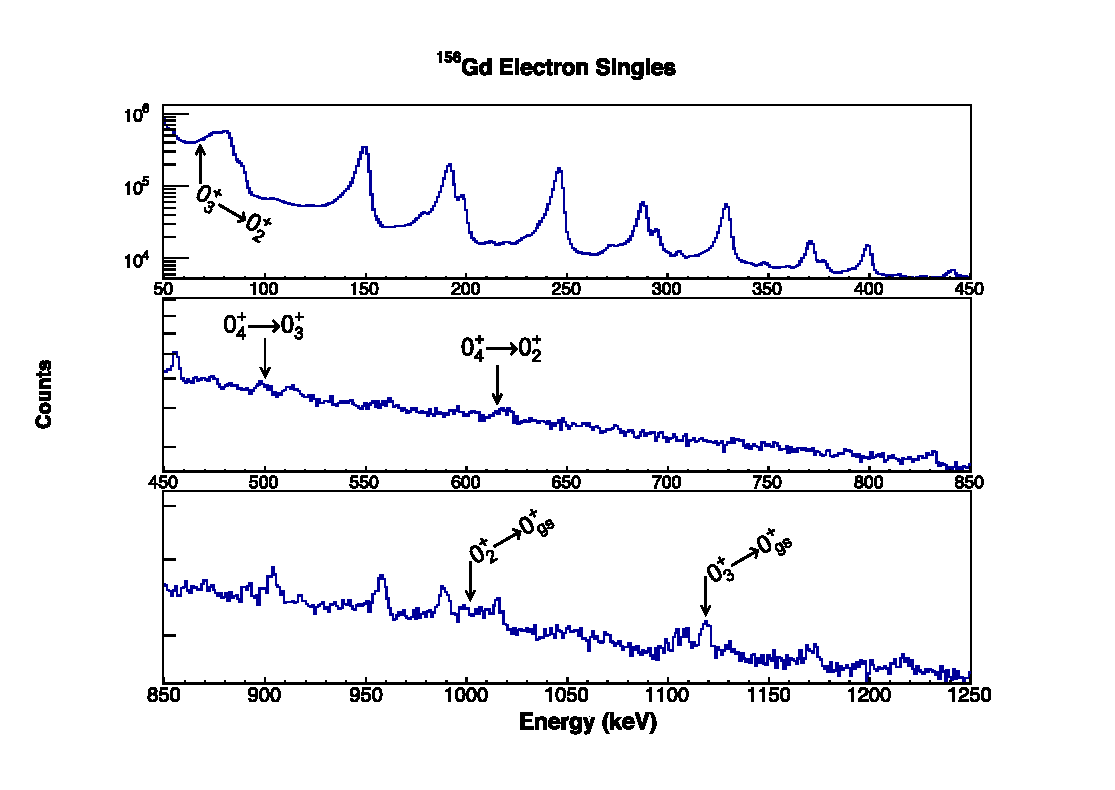
\includegraphics[scale=0.8]{156GdTablesAndFigs/156Gd_Singles_Electron_Label.eps}
    \caption{Electron singles for $^{156}$Gd. The energies of transitions between $0^+$ states are marked in the plot.}
    \label{fig:156_e_singles}
\end{figure}

To obtain information in these areas, and for possible $J^{\pi}\rightarrow J^{\pi}$ transitions, energy gates were used. A full list of gates and spectra can be found in Appendix \ref{chap:156_spectra}.

\subsection{$J^{\pi}\rightarrow J^{\pi}$ Transitions}

After identification of the bands and transitions, gates were put on the incoming and outgoing transitions of states of interest, namely even-$J^+$ states. Incoming transitions did not have enough statistics to yield information. For the $0^+$ states, this is unfortunate, as only incoming transitions can be used for transitions to the ground state. Outgoing transitions had more statistics, and results could be obtained.  To look for these transitions of interest, other transitions, namely those of the ground state band, were subtracted from the regions of interest as described in Section \ref{sec:upper_limit}. This subtraction technique causes the results to be treated as limits.  $J^\pi\rightarrow J^\pi$ transitions up to $4^+$ were seen. Tables \ref{tab:156Gd_0_to_0}, \ref{tab:156Gd_2_to_2}, and \ref{tab:156Gd_4_to_4} are the tabulated results. These values are compared with Konijn\citep{konijn81:_156gd} where available. Additionally, the theoretical conversion coefficients have been listed for the $M1$ and $E2$ transitions, as taken from BrIcc\citep{kibedi08:_BRICC}.
    
\afterpage{\clearpage\begin{landscape}
    \begin{longtable}{c|c|c|c|c|c|c|c|c}
        \caption{$0^+\rightarrow 0^+$ Transitions in $^{156}$Gd}
        \label{tab:156Gd_0_to_0}\\
        \toprule
        &	& & & 	&  &	& \multicolumn{2}{c}{Theory}	\\
        $E_i$ (keV)	& Band &	$E_f$ (keV)	& Band &$E$ (keV)	&	Gate &		$\alpha$ (This Work)	& $\alpha$(M1) & $\alpha$(E2) \\
        \hline
        \endfirsthead
        \toprule
        \caption[]{$0^+\rightarrow 0^+$ Transitions in $^{156}$Gd}\\
        & & &	& 	&  &	& \multicolumn{2}{c}{Theory}	\\
        $E_i$ (keV)	& Band &	$E_f$ (keV)	& Band &$E$ (keV)	&	Gate &		$\alpha$ (This Work)	& $\alpha$(M1) & $\alpha$(E2) \\
	    \endhead
	    \endfoot
	    \multicolumn{9}{p{1.4\textwidth}}{A list of conversion coefficients from $^{156}$Gd for $0^+\rightarrow 0^+$ transitions seen in the gated data. All listed theoretical values are for the K-shell internal conversion coefficient. Numbers are compared with theoretical values for illustration. All coefficients are K-shell electrons. }
	    \endlastfoot
        1168.186 & $0^+_{3}$ & 1049.487  & $0^+_{2}$ & 118.71 &  960.50771 & $>1.1970$ & 1.042 (15) & 0.726 (11) \\
        \bottomrule
    \end{longtable}
\end{landscape}}

\afterpage{\clearpage\begin{landscape}
    \begin{longtable}{c|c|c|c|c|c|c|c|c|c}
        \caption{$2^+\rightarrow 2^+$ Transitions in $^{156}$Gd}
        \label{tab:156Gd_2_to_2}\\
        \toprule
        & & &	& 	&  &	& \multicolumn{2}{c|}{Theory\citep{kibedi08:_BRICC}}	& 	\\
        $E_i$ (keV)	& Band &	$E_f$ (keV)	& Band &$E$ (keV)	&	Gate &		$\alpha$ (This Work)	& $\alpha$(M1) & $\alpha$(E2) &	$\alpha$ (Konijn)	\\
        \hline
        \endfirsthead
        \toprule
        \caption[]{$2^+\rightarrow 2^+$ Transitions in $^{156}$Gd}\\
        & & &	& 	&  &	& \multicolumn{2}{c|}{Theory\citep{kibedi08:_BRICC}}	& 	\\
        $E_i$ (keV)	& Band &	$E_f$ (keV)	& Band &$E$ (keV)	&	Gate &		$\alpha$ (This Work)	& $\alpha$(M1) & $\alpha$(E2) &	$\alpha$ (Konijn)	\\
        \hline
	    \endhead
	    \endfoot
	    \multicolumn{10}{p{1.4\textwidth}}{A list of conversion coefficients from $^{156}$Gd for $2^+\rightarrow 2^+$ transitions seen in the gated data. All listed theoretical values are for the K-shell internal conversion coefficient. Numbers are compared with Konijn et al.\citep{konijn81:_156gd} All coefficients are K-shell electrons. }
	    \endlastfoot
        1258.075 & $0^+_{3}$ & 1129.437 & $0^+_{2}$ & 128.638 & 1040.470 & $>0.5325$ & 0.830 (12) & 0.578 (8) &\\ \hline
        1258.075 & $0^+_{3}$ & 1154.152 & $\gamma$ & 103.92 & 1065.1781 & $>2.9695$ & 1.524 (22)  & 1.049 (15) &\\ \hline
        1827.841 & $2^+_2$ & 1129.437 & $0^+_{2}$ & 698.407 & 1040.470 & $<0.0208$ & 0.00932 (13) & 0.00506 (7) & \\ \hline
        1827.841 & $2^+_2$ & 1154.152 & $\gamma$ & 673.684 & 1065.1781 & $<0.0228$ & 0.01018 (15) & 0.00550 (8) &\\ \hline
        1827.841 & $2^+_2$ & 1258.075 & $0^+_{3}$ & 569.771 & 1169.087 & $<0.0013$ & 0.01545 (22) & 0.00819 (12) & 0.006 (4) \\
        \bottomrule
    \end{longtable}
\end{landscape}}

\afterpage{\clearpage\begin{landscape}
    \begin{longtable}{c|c|c|c|c|c|c|c}
        \caption{$4^+\rightarrow 4^+$ Transitions in $^{156}$Gd}
        \label{tab:156Gd_4_to_4}\\
        \toprule
        &	& 	&  &	& \multicolumn{2}{c}{Theory}	& 	\\
        $E_i$ (keV)	&	$E_f$ (keV)	& $E$ (keV)	&	Gate &		$\alpha$ (This Work)	& $\alpha$(M1) & $\alpha$(E2) &	$\alpha$ (Konijn)	\\
        \hline
        \endfirsthead
        \toprule
        \caption[]{$4^+\rightarrow 4^+$ Transitions in $^{156}$Gd}\\
        &	& 	&  &	& \multicolumn{2}{c}{Theory}	& 	\\
        $E_i$ (keV)	&	$E_f$ (keV)	& $E$ (keV)	&	Gate &		$\alpha$ (This Work)	& $\alpha$(M1) & $\alpha$(E2) &	$\alpha$ (Konijn)	\\
        \hline
	    \endhead
        1462.297 & 1297.822 & 164.469 & 1009.649 & $>0.4870$ & 0.416 (6) & 0.279 (4) & \\ \hline
        1462.297 & 1355.422 & 106.88 & 1067.2325 & $>0.7233$ & 1.405 (20) & 0.972 (14) & \\ \hline
        1510.594 & 1297.822 & 212.771 & 1009.649 & $>0.0704$  & 0.204 (3) & 0.1282 (18) & \\ \hline
        1510.594 & 1355.422 & 155.168 & 1067.2325 & $>0.0981$ & 0.490 (7) & 0.333 (5) &  \\
        \bottomrule
    \end{longtable}
    \caption{A list of conversion coefficients from $^{156}$Gd for $4^+\rightarrow 4^+$ transitions seen in the gated data. All listed theoretical values are for the K-shell internal conversion coefficient. Numbers are compared with Konijn et al. \citep{konjin81:_156gd} All coefficients are K-shell electrons.}
\end{landscape} }

Due to the lack of lifetimes of these states, $B(E0)$ values cannot be calculated. However, the relative intensities of these values can be compared, assuming they are coming from the same state, as the lifetime would divide out (see equations \ref{eq:rho_life} and \ref{eq:BE0}). The contributions from the individual components of the transition must be separated out for the $2^+$ and $4^+$ transitions. This was done by getting the $q^2$ values multiplied by the theoretical $\alpha(E2)$, which gives an estimate of $E0$ intensity (see Section \ref{sec:E0}). None of the transitions have known $\delta$ mixing ratios, so $\delta$ was assumed to be 1, and the theoretical mixed $M1$ and $E2$ $\alpha$ was subtracted. In some cases, this left a negative value, which has been excluded from the table of results, Table \ref{tab:156Gd_E0}. All values calculated are upper or lower limits, as the $\alpha$ calculated in the previous tables were upper and lower limits. 

With these values, two transitions from the same level can be compared using the $B(E0)$ formula to take the energy adjustment into account. It is also adjusted by the ratio of the gate efficiencies. Only one $2^+$ level had transitions to other $2^+$ states that could be compared. This ratio is in Table \ref{tab:156Gd_BE0_Comp}.

The first excited $0^+$ band and the $\gamma$ band are not discussed, as no $J^{\pi}\rightarrow J^{\pi}$ transitions could be observed leaving these levels.

\afterpage{\begin{portrait}
    \begin{longtable}{c|c|c|c|c}
        \caption{$E0$ Contributions for $J^{\pi}\rightarrow J^{\pi}$ Transitions}
        \label{tab:156Gd_E0}\\
        \toprule
        $E_i$ (keV)	&	$E_f$ (keV)	& $E$ (keV)	&	Gate &		$q^2\alpha(E2)$		\\
        \hline
        \endfirsthead
        \toprule
        \caption{$E0$ Contributions for $J^{\pi}\rightarrow J^{\pi}$ Transitions} \\
        $E_i$ (keV)	&	$E_f$ (keV)	& $E$ (keV)	&	Gate &		$q^2\alpha(E2)$		\\
        \hline
	    \endhead
	    \multicolumn{5}{l}{$0^+\rightarrow 0^+$} 	\\ \hline
        1168.186 & 1049.187 &  118.71 & 960.50771 & $>0.626$ \\\hline
        \multicolumn{5}{l}{$2^+\rightarrow 2^+$} 	\\ \hline
        1258.075 & 1154.152 & 103.92 & 1065.1781 & $>3.366$  \\ \hline
        1827.841 & 1129.437 & 698.407 & 1040.47 & $<0.02722$  \\ \hline
        1827.841 & 1154.152 & 673.684 & 1065.1781 & $<0.02992$  \\ \hline
        \multicolumn{5}{l}{$4^+\rightarrow 4^+$} 	\\ \hline
        1462.297 & 1297.822 & 164.469 & 1009.649 &  $>0.279$  \\
        \bottomrule
	\end{longtable}
    \item{A list of E0 contributions in $^{156}Gd$. These values have not been normalized, as the lifetime of the states are unknown. The $0^+\rightarrow 0^+$ transitions list the $\alpha(expt)$, as $M1$ and $E2$ transitions are forbidden. Table \ref{tab:156Gd_BE0_Comp} compares values between two transitions of the same initial state. Only non-negative values are listed in the table, and $\delta$ was assumed to be 1, as no mixing ratios are known for these transitions. For $\alpha(exp)$, $\alpha(M1)$, and $\alpha(E2)$ used in these calculations, please refer to Tables \ref{tab:156Gd_0_to_0}-\ref{tab:156Gd_4_to_4}.}
\end{portrait}}

\afterpage{
    \begin{longtable}{c|c|c|c|c|c|c}
        \caption{$B(E0)$ Ratios for $J^{\pi}\rightarrow J^{\pi}$ Transitions}
        \label{tab:156Gd_BE0_Comp}\\
        \toprule
        $E_i$ (keV)	& Band &	$E_{0^+_2}$ (keV)	& Gate$_{0^+_2}$ & $E_{\gamma}$ (keV)	& Gate$_{\gamma}$ &	$B(E0)$	Ratio	\\
        \hline
        \endfirsthead
        \toprule
        \caption{$B(E0)$ Ratios for $J^{\pi}\rightarrow J^{\pi}$ Transitions} \\
        $E_i$ (keV)	& Band &	$E_{0^+_2}$ (keV)	& Gate$_{0^+_2}$ & $E_{\gamma}$ (keV)	& Gate$_{\gamma}$ &	$B(E0)$	Ratio	\\
        \hline
	    \endhead
	    \endfoot
	    \multicolumn{7}{p{\textwidth}}{Ratios of the $B(E0)$ values in $^{156}$Gd. Only ratios between two transitions of the same state are listed, as the lifetime of the states are unknown. Table \ref{tab:156Gd_E0} lists the values that were used in the calculation. The gates are included, as an efficiency correction was made on the ratio based on the gates. In many cases, only upper or lower limits for the values could be used for this calculation. Errors are not given on these values.}
	    \endlastfoot
        \multicolumn{6}{l}{$2^+\rightarrow 2^+$} 	\\ \hline
        1827.841 & $2^+_2$ & 1129.437 & 1040.47 & 1154.152 & 1065.1781 & 1.128  \\
        \bottomrule
	\end{longtable}
}

\subsubsection{$K^{\pi}=0^+_3$, Second Excited $0^+$ Band, 1168.186 keV}

Transitions from this band to both the first $0^+$ band ($0^+_{2}$) and the $\gamma$ band could be observed. All values observed are lower limits. The $0^+$ state in the band has a known lifetime, allowing for the $0^+_3\rightarrow 0^+_2$ nuclear matrix element to the first excited $0^+$ state be calculated\citep{aprahamian18:_156gd}. Table \ref{tab:156Gd_E0_0} contains the calculated $q^2$ and $\rho^2$ value for the $0^+_3\rightarrow0^+_2$ transition.

\afterpage{\begin{landscape}
\begin{table}
    \caption{$E0$ Contributions for $J^{\pi}\rightarrow J^{\pi}$ Transitions}
        \label{tab:156Gd_E0_0}
    \begin{tabular}{>{\footnotesize}c|>{\footnotesize}c|>{\footnotesize}c|>{\footnotesize}c|>{\footnotesize}c|>{\footnotesize}c|>{\footnotesize}c|>{\footnotesize}c}
        \toprule
        $E_i$ (keV)	& Transition & $E0$ (keV)	& Transition & $E2$ (keV)	&	$t_{1/2}$ (ps) & $q_K^2(E0/E2)$	& $\rho^2$(E0)	\\
        \hline
        1168.186 & $0^+_3\rightarrow0^+_2$ & 118.71 & $0^+_3\rightarrow2^+_{gs}$ & 1079.216 & $0.9031<t_{1/2}<4.4221$ & 1.995 (15) & $22.78<\rho^2<111.53$ \\
        \bottomrule
        \multicolumn{8}{p{1.4\textwidth}}{Table \ref{tab:156Gd_E0_0}: A list of $q_K^2(E0/E2)$ and $\rho^2$(E0) contributions in $^{156}$Gd for the $0^+\rightarrow0^+$ transitions. Lifetime from \citep{aprahamian18:_156gd}.}
	\end{tabular}
\end{table}
\end{landscape}
}

For the other transitions to the first excited $0^+$ band, the $2^+_{0^+_3}\rightarrow 2^+_{0^+_2}$ transition lower limit did not allow for any conclusions to be drawn as to the nature of the transition. The $4^+_{0^+_3}\rightarrow 4^+_{0^+_2}$ transition lower limit indicates an E0 component. Assuming both transitions have an E0 component and $\delta$ is 1, Table \ref{tab:156Gd_E0} has the lower limits tabulated for the $q^2\alpha$(E2) values.

For the transitions to the $\gamma$ band, the $2^+_{0^+_3}\rightarrow 2^+_{0^+_2}$ transition lower limit indicates an E0 component. The $4^+_{0^+_3}\rightarrow 4^+_{0^+_2}$ transition lower limit did not allow for any conclusions to be drawn as to the nature of the transition.

\subsubsection{$K^{\pi}=2^+_2$, Second Excited $2^+$ Band, 1827.841 keV}

The transitions from the head of this band to the $2^+$ states of the $\gamma$ band and the first and second $0^+$ excited states were observed. All three coefficients are upper limits. The transitions to the $\gamma$ band and the first excited $0^+$ band may have E0 components, as the upper limits do not rule them out. Assuming both transitions have an E0 component and $\delta$ is 1, Table \ref{tab:156Gd_E0} has the upper limits tabulated for the $q^2\alpha$(E2) values. The values are quite small. Table \ref{tab:156Gd_BE0_Comp} compares the strengths of the two transitions as a ratio. The ratio is close to 1, indicating similar transition strengths from this $2^+$ excited band to the $\gamma$ band the first excited $0^+$ band.

The upper limit on the transition to the second excited $0^+$ band does rule out an E0 component. The upper limit is lower than the measurement by Konijn, although not significantly so when looking at the error on the conversion coefficient\citep{konijn81:_156gd}.

\subsubsection{$K^{\pi}=4^+_1$, First Excited $4^+$ Band, 1510.594 keV}

The transitions from the head of this band to the $4^+$ states of the $\gamma$ band and the first excited state were observed. Both coefficients are lower limits. No conclusions can be drawn for the transitions, as the lower limits do not rule any type of transition out.